% Презентация к ВКР магистра. xelatex + beamer.
% Сборка:  latexmk -xelatex main.tex
% Структура — каноничный формат защиты МАИ:
%   проблема → область → актуальность/противоречия → цель/задачи →
%   объект/предмет/предположение → посылки → методы → результаты (превью) →
%   формальная постановка → ТЗ → система качества → архитектура → алгоритмы →
%   данные → главные числа → демо → значимость → достоверность →
%   рекомендации → оперативный эффект → заключение (таблица) → спасибо.
%
% Картинки — из общей media-library ../images/ (та же, что у report/).

\documentclass[aspectratio=169, 14pt]{beamer}

\usepackage{fontspec}
\setmainfont{Times New Roman}
\setsansfont{Arial}
\setmonofont{Courier New}

\usepackage[english,russian]{babel}
\usepackage{amssymb,amsmath,mathtools}
\usepackage{graphicx}
\usepackage{booktabs}
\usepackage{colortbl}  % для \rowcolor в таблице headline
\usepackage{tikz}
\usetikzlibrary{arrows.meta, positioning, fit, backgrounds, calc, shapes.geometric}

% Аналог appendixnumberbeamer: исключаем бэкап-слайды из total.
\newcommand{\backupbegin}{%
  \newcounter{finalframe}%
  \setcounter{finalframe}{\value{framenumber}}%
}
\newcommand{\backupend}{%
  \setcounter{framenumber}{\value{finalframe}}%
}
\graphicspath{{../images/}}

% Минималистичная тема + навигационная полоска секций сверху.
\usetheme{default}
\usecolortheme{seahorse}
\useoutertheme[subsection=false]{miniframes}
\setbeamertemplate{navigation symbols}{}
\setbeamercolor{frametitle}{fg=black}
\setbeamerfont{frametitle}{series=\bfseries}

% Кастомный footline: подпись слева + N / total справа.
\setbeamertemplate{footline}{%
  \leavevmode%
  \hbox{%
    \begin{beamercolorbox}[wd=.55\paperwidth,ht=2.5ex,dp=1ex,leftskip=1.2em]{author in head/foot}%
      \fontsize{7pt}{8pt}\selectfont\itshape\color{black!55}%
      ВКР магистра Фролова М.А.%
    \end{beamercolorbox}%
    \begin{beamercolorbox}[wd=.45\paperwidth,ht=2.5ex,dp=1ex,rightskip=1.2em]{author in head/foot}%
      \hfill\fontsize{8pt}{9pt}\selectfont\color{black!70}%
      \insertframenumber\,/\,\inserttotalframenumber%
    \end{beamercolorbox}%
  }%
  \vskip0pt%
}

% Подсветка зелёным для положительных дельт в таблицах.
\definecolor{posgreen}{RGB}{0,128,0}
\newcommand{\pos}[1]{{\color{posgreen}#1}}

% Реквизиты титула вынесены в отдельный файл.
% Заголовок и реквизиты для титульного слайда. Подключается из main.tex
% через % Заголовок и реквизиты для титульного слайда. Подключается из main.tex
% через % Заголовок и реквизиты для титульного слайда. Подключается из main.tex
% через \input{titlepage} в преамбуле перед \begin{document}.

\title[Гибридное обогащение каталога]%
      {Система автоматизированного обогащения товарных данных\\
       для интернет-магазина}

\author{Фролов М.~А.}

\institute[МАИ, Институт~№~8]%
          {Московский авиационный институт (национальный исследовательский университет)\\
           Институт~№~8 «Компьютерные науки и прикладная математика»\\
           Образовательный центр Института~№~8\\[0.3em]
           Выпускная квалификационная работа\\[0.2em]
           Программа «Продуктовая разработка и разработка программных систем»\\[0.3em]
           Научный руководитель: Судаков В.~А., д.\,т.\,н., профессор образовательного центра Института~№~8}

\date{Москва, \the\year}
 в преамбуле перед \begin{document}.

\title[Гибридное обогащение каталога]%
      {Система автоматизированного обогащения товарных данных\\
       для интернет-магазина}

\author{Фролов М.~А.}

\institute[МАИ, Институт~№~8]%
          {Московский авиационный институт (национальный исследовательский университет)\\
           Институт~№~8 «Компьютерные науки и прикладная математика»\\
           Образовательный центр Института~№~8\\[0.3em]
           Выпускная квалификационная работа\\[0.2em]
           Программа «Продуктовая разработка и разработка программных систем»\\[0.3em]
           Научный руководитель: Судаков В.~А., д.\,т.\,н., профессор образовательного центра Института~№~8}

\date{Москва, \the\year}
 в преамбуле перед \begin{document}.

\title[Гибридное обогащение каталога]%
      {Система автоматизированного обогащения товарных данных\\
       для интернет-магазина}

\author{Фролов М.~А.}

\institute[МАИ, Институт~№~8]%
          {Московский авиационный институт (национальный исследовательский университет)\\
           Институт~№~8 «Компьютерные науки и прикладная математика»\\
           Образовательный центр Института~№~8\\[0.3em]
           Выпускная квалификационная работа\\[0.2em]
           Программа «Продуктовая разработка и разработка программных систем»\\[0.3em]
           Научный руководитель: Судаков В.~А., д.\,т.\,н., профессор образовательного центра Института~№~8}

\date{Москва, \the\year}


\begin{document}

% ===========================================================================
% Slide 0 — TITLE
% ===========================================================================
{
    \setbeamertemplate{footline}{}  % убрать номер на титуле
    \begin{frame}[plain]
        \titlepage
    \end{frame}
}

% ===========================================================================
\section{Актуальность}
% ===========================================================================

% --- Slide: Проблемные вопросы практики ----------------------------------
\begin{frame}{Проблемные вопросы практики обогащения карточек}
\begin{columns}[T]
\column{0.55\textwidth}
\fontsize{11pt}{14pt}\selectfont
\begin{itemize}
    \setlength{\itemsep}{0.4em}
    \item Каталоги маркетплейсов — \textbf{десятки миллионов SKU}.
    \item Партнёры присылают \textbf{лишь базовый набор} полей.
    \item PIM-системы \textbf{хранят}, но \textbf{не извлекают} атрибуты.
    \item Ручное заполнение — \textbf{узкое место} вывода ассортимента.
\end{itemize}

\vspace{0.6em}
\fontsize{10pt}{12pt}\selectfont\itshape\color{black!65}
$\sim$10\textsuperscript{7} SKU \quad$\cdot$\quad часы на карточку
\quad$\cdot$\quad линейная стоимость от объёма

\column{0.43\textwidth}
\centering
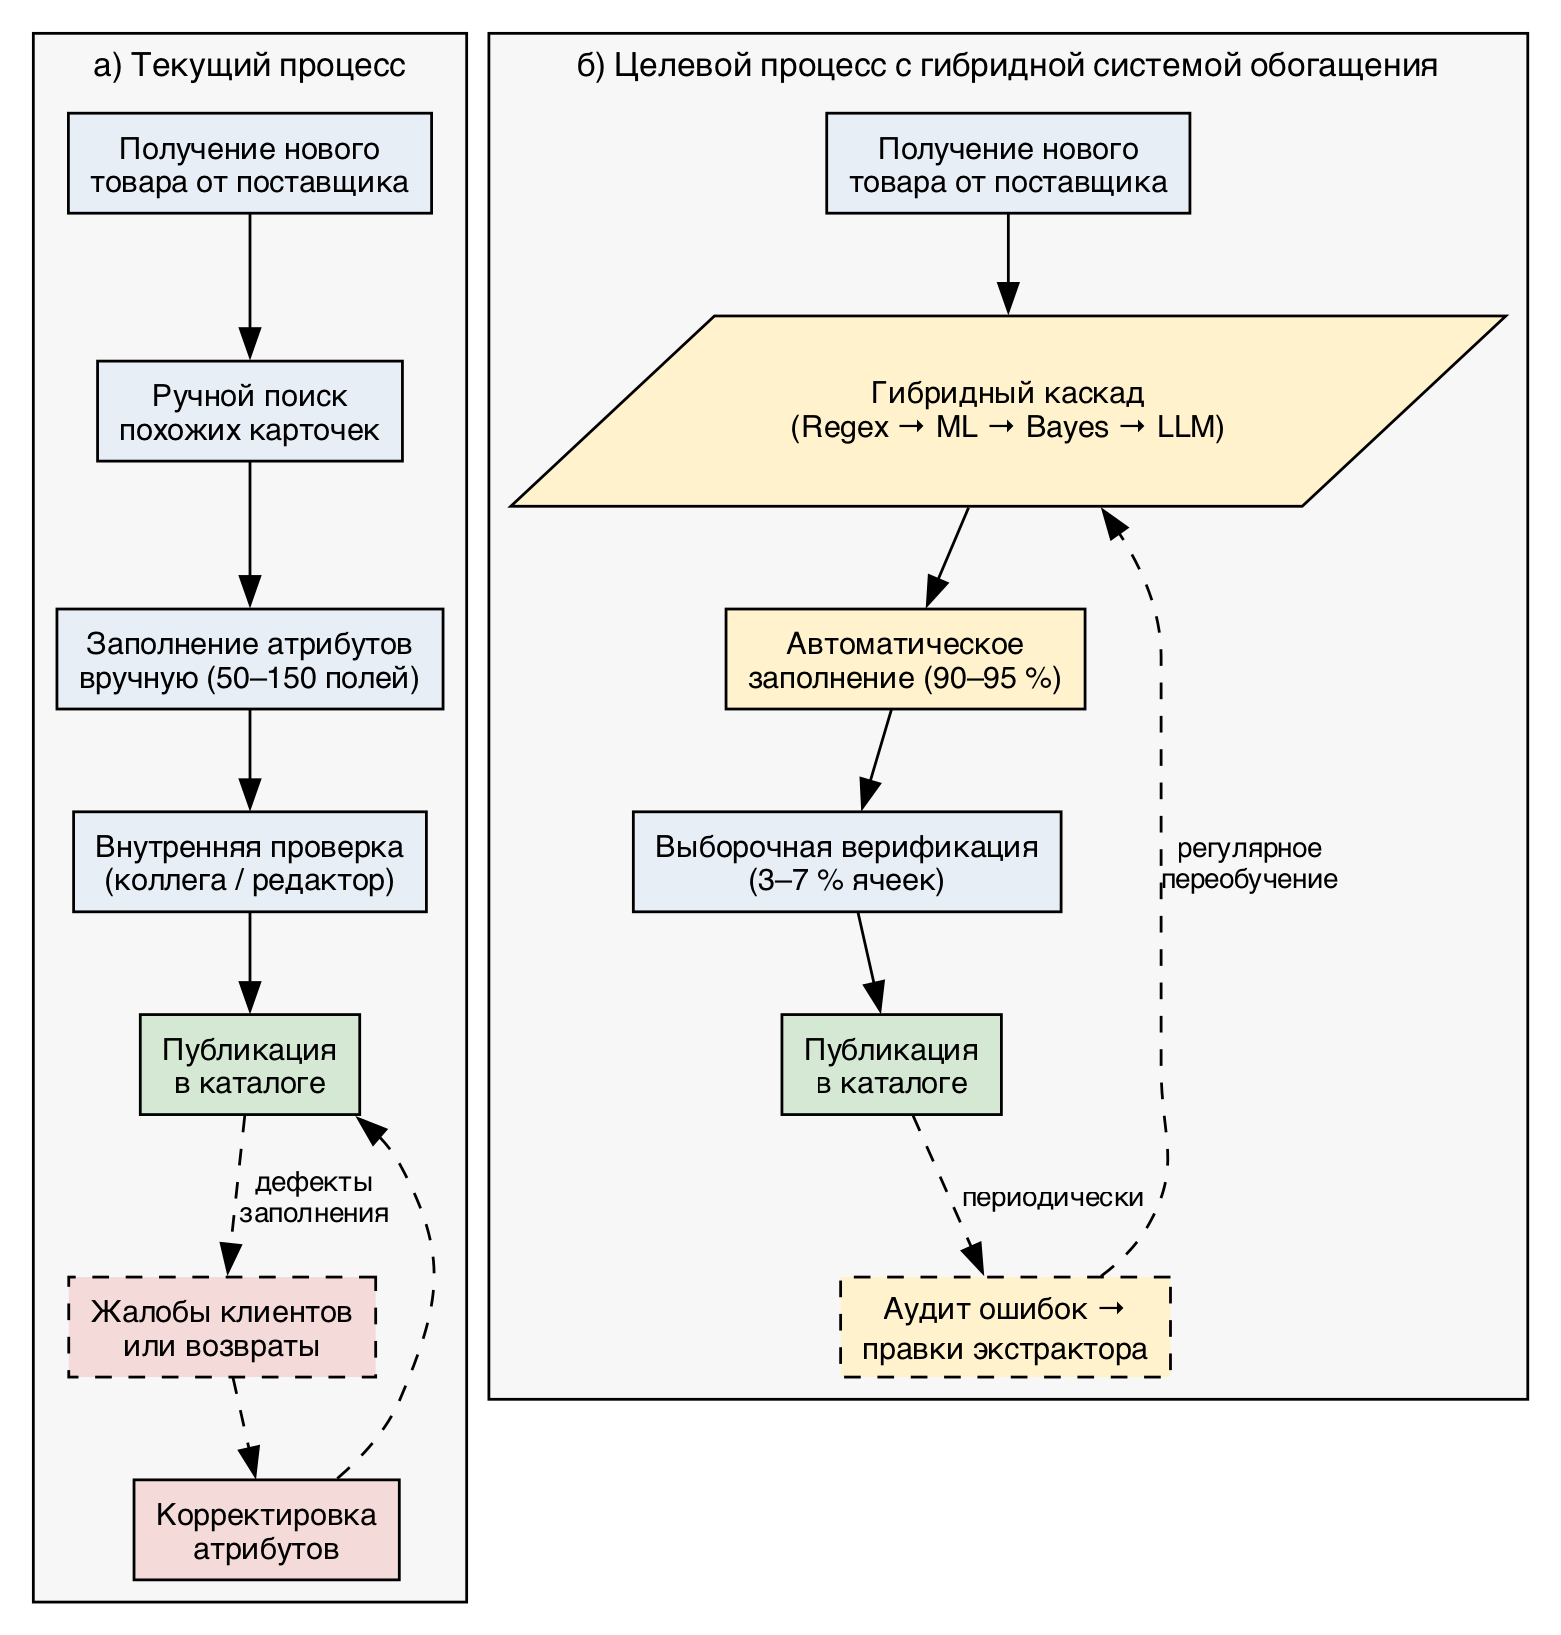
\includegraphics[height=5.6cm]{fig_1_1_cm_process.png}\\[0.2em]
\fontsize{7pt}{9pt}\selectfont\itshape\color{black!60}
Процесс контент-менеджера: текущий $\to$ целевой
\end{columns}
\end{frame}

% --- Slide: Область и направление исследования ---------------------------
\begin{frame}{Область и направление исследования}
\fontsize{12pt}{15pt}\selectfont
\textbf{Область.} Обогащение карточек товаров в интернет-магазинах:
преобразование партнёрских полей в структурированные атрибуты.

\vspace{0.8em}
\textbf{Направление.} \textbf{Гибридная каскадная система} извлечения атрибутов:
регулярные выражения + ML с калиброванной уверенностью + LLM-fallback,
интеграция рядом с PIM.

\vspace{1.2em}
\fontsize{11pt}{13pt}\selectfont\itshape\color{black!65}
\centering
$\Rightarrow$ перенос акцента с «одна большая LLM на всё» на\\
\textbf{поатрибутную маршрутизацию} между слоями разной стоимости.
\end{frame}

% --- Slide: Актуальность ВКР (противоречия + задача) ---------------------
\begin{frame}{Актуальность направления и задача ВКР}
\fontsize{10pt}{13pt}\selectfont
\textbf{Противоречия}
\begin{itemize}
    \setlength{\itemsep}{0.15em}
    \item \textbf{Процесс} — 10\textsuperscript{7}+ SKU vs пропускная способность контент-менеджеров.
    \item \textbf{Средства} — PIM хранит, но не извлекает атрибуты.
    \item \textbf{Технология} — точность LLM vs её \textbf{цена} на промышленных объёмах.
\end{itemize}

\vspace{0.5em}
\textbf{Что есть для разрешения}
\begin{itemize}
    \setlength{\itemsep}{0.05em}
    \item Многоязычные эмбеддинги (\texttt{sentence-transformers}, 50+ языков).
    \item Калиброванные классификаторы (XGBoost + Platt/isotonic).
    \item Открытые LLM (gpt-oss-120b, Ollama) — локальное развёртывание.
    \item Открытый корпус Open Food Facts (4{,}5\,млн SKU).
\end{itemize}

\vspace{0.5em}
\textbf{Задача ВКР.} Программное средство обогащения товарных данных
с заданной точностью при \textbf{кратном сокращении стоимости} vs прямой вызов LLM
и локальным развёртыванием.
\end{frame}

% --- Slide: Аналоги ------------------------------------------------------
\begin{frame}{Аналоги: пробел в существующих подходах}
\centering
\fontsize{9pt}{11pt}\selectfont
\setlength{\tabcolsep}{4pt}
\begin{tabular}{l c c c c c}
\toprule
\textbf{Критерий} & \textbf{TXtract} & \textbf{MAVE} & \textbf{FrugalGPT} & \textbf{AutoMix} & \textbf{Наша система} \\
\midrule
Per-attribute policy           & \checkmark & \checkmark & \textendash & \textendash & \pos{\checkmark} \\
Калиброванный отказ от ответа  & \textendash & \textendash & \textendash & \checkmark & \pos{\checkmark} \\
Cost-aware routing             & \textendash & \textendash & \checkmark & \checkmark & \pos{\checkmark} \\
Brand-disjoint evaluation      & \textendash & \textendash & \textendash & \textendash & \pos{\checkmark} \\
Гибридный backend (regex+ML+LLM)& \textendash & \textendash & \textendash & \textendash & \pos{\checkmark} \\
Локальное развёртывание         & \checkmark & \checkmark & \textendash & \textendash & \pos{\checkmark} \\
\bottomrule
\end{tabular}
\vspace{0.5em}

\fontsize{10pt}{12pt}\selectfont
Ни одна из существующих систем не объединяет \textbf{per-attr policy},
\textbf{проверку на непересекающихся брендах} и \textbf{гибридный backend} одновременно.
\end{frame}

% ===========================================================================
\section{Цель и задачи}
% ===========================================================================

% --- Slide: Цель и задачи ВКР --------------------------------------------
\begin{frame}{Цель и задачи ВКР}
\fontsize{11pt}{13pt}\selectfont
\textbf{Цель.} Программное средство обогащения товарных данных на основе
гибридной каскадной архитектуры.

\vspace{0.5em}
\textbf{Частные задачи}
\begin{enumerate}
    \setlength{\itemsep}{0.2em}
    \item Анализ существующих подходов, выявление пробела.
    \item Функциональные, нефункциональные, архитектурные требования; интегральный критерий качества.
    \item Каскад из 4 слоёв + поатрибутная политика маршрутизации.
    \item Реализация end-to-end демо-комплекса (REST API + Web-UI).
    \item Pre-registered протокол оценки на выборке с непересекающимися брендами.
    \item Рекомендации по внедрению и эксплуатации.
\end{enumerate}
\end{frame}

% --- Slide: Объект, предмет, рабочее предположение -----------------------
\begin{frame}{Объект, предмет и рабочее предположение}
\fontsize{11pt}{14pt}\selectfont
\textbf{Объект.} Процессы обогащения карточек товаров в интернет-магазинах.

\vspace{0.5em}
\textbf{Предмет.} Методы и алгоритмы извлечения атрибутов, политики
маршрутизации между слоями разной стоимости и протоколы их оценки.

\vspace{0.8em}
\textbf{Рабочее предположение.}\\[0.2em]
\fontsize{10pt}{13pt}\selectfont
Каскад из регулярных выражений, ML с калиброванной уверенностью,
байесовской валидации и LLM-fallback с \textbf{поатрибутной политикой эскалации}
обеспечивает заданную точность обогащения при \textbf{кратном сокращении стоимости}
vs прямой вызов LLM и допускает локальное развёртывание.
\end{frame}

% --- Slide: Исходные посылки ---------------------------------------------
\begin{frame}{Исходные посылки}
\fontsize{11pt}{13pt}\selectfont
\begin{columns}[T]
\column{0.5\textwidth}
\textbf{1. Унаследованная инфраструктура}\\[0.2em]
\fontsize{10pt}{12pt}\selectfont
PIM (Akeneo, Pimcore, Salsify) хранит, но не извлекает атрибуты.

\vspace{0.7em}
\fontsize{11pt}{13pt}\selectfont
\textbf{2. Теоретическая основа}\\[0.2em]
\fontsize{10pt}{12pt}\selectfont
Многоязычные эмбеддинги, калиброванная классификация (Platt + isotonic),
байесовские сети, prompt-инженерия (few-shot, schema-constrained).

\column{0.5\textwidth}
\textbf{3. Технологический стек}\\[0.2em]
\fontsize{10pt}{12pt}\selectfont
Python / FastAPI / Go-gateway / React; Docker-compose;
XGBoost, sentence-transformers, pgmpy; Ollama для локальной LLM.

\vspace{0.7em}
\fontsize{11pt}{13pt}\selectfont
\textbf{4. Открытые данные}\\[0.2em]
\fontsize{10pt}{12pt}\selectfont
Open Food Facts (4{,}5\,млн SKU, $\sim$40\,\% FR / 10\,\% EN / 7\,\% DE)
+ открытые источники по электронике для cold-start.
\end{columns}
\end{frame}

% --- Slide: Методы исследования ------------------------------------------
\begin{frame}{Методы исследования}
\fontsize{11pt}{14pt}\selectfont
\begin{columns}[T]
\column{0.48\textwidth}
\textbf{Системный анализ}\\
\fontsize{10pt}{12pt}\selectfont
Декомпозиция процесса, выявление противоречий.

\vspace{0.6em}
\fontsize{11pt}{14pt}\selectfont
\textbf{Управление требованиями}\\
\fontsize{10pt}{12pt}\selectfont
ФР\,/\,НФР\,/\,А-требования, интегральный критерий $Q$.

\vspace{0.6em}
\fontsize{11pt}{14pt}\selectfont
\textbf{Машинное обучение}\\
\fontsize{10pt}{12pt}\selectfont
Эмбеддинги + XGBoost, калибровка Platt\,+\,isotonic.

\column{0.48\textwidth}
\textbf{Промпт-инженерия}\\
\fontsize{10pt}{12pt}\selectfont
Few-shot со схемой ответа, селективная эскалация.

\vspace{0.6em}
\fontsize{11pt}{14pt}\selectfont
\textbf{Pre-registered эксперимент}\\
\fontsize{10pt}{12pt}\selectfont
Brand-disjoint, McNemar + Бонферрони, Wilson 95\,\% CI.

\vspace{0.6em}
\fontsize{11pt}{14pt}\selectfont
\textbf{Итеративная разработка}\\
\fontsize{10pt}{12pt}\selectfont
Цикл аудит\,$\to$\,правки\,$\to$\,переобучение\,$\to$\,измерение.
\end{columns}
\end{frame}

% --- Slide: Основные результаты работы (превью) --------------------------
\begin{frame}{Основные результаты работы}
\fontsize{11pt}{14pt}\selectfont
\begin{enumerate}
    \setlength{\itemsep}{0.4em}
    \item \textbf{Требования и качество:} 6 ФР, 4 НФР, 3 А; критерий $Q$ с 4 показателями.
    \item \textbf{Методика:} 4-слойный каскад с поатрибутной политикой эскалации.
    \item \textbf{Архитектура:} REST-микросервис, упакованный в \texttt{docker-compose}.
    \item \textbf{Реализация:} $\sim$15\,тыс. строк Python, 22 пары «категория-атрибут», работающий e2e демо.
    \item \textbf{Оценка} ($n{=}3257$): cascade-only \textbf{94{,}8\,\%} micro\,/\,\textbf{0{,}899} macro-F1;
          E2E production-realistic \textbf{91{,}1\,\%}; \pos{$\div$14} стоимости vs all-LLM.
\end{enumerate}
\end{frame}

% ===========================================================================
\section{Постановка}
% ===========================================================================

% --- Slide: Формальная постановка задачи ---------------------------------
\begin{frame}{Формальная постановка задачи}
\fontsize{11pt}{14pt}\selectfont
\textbf{Вход:} $x = (\texttt{product\_name},\ \texttt{brands},\ \texttt{ingredients\_text},\ \texttt{quantity},\ \texttt{code})$.

\vspace{0.4em}
\textbf{Политика обогащения:}
\[
    \pi: x \;\longrightarrow\; (a,\ \hat y,\ c,\ \ell)
\]
$a$ — атрибут, $\hat y$ — значение, $c{\in}[0,1]$ — \textbf{калиброванная} уверенность,
$\ell$ — слой-источник.

\vspace{0.7em}
\textbf{Метрики:}
\begin{itemize}
    \fontsize{10pt}{13pt}\selectfont
    \setlength{\itemsep}{0.15em}
    \item $\mathrm{Acc}(\pi)$ на проверке с непересекающимися брендами.
    \item $C(\pi)$ — стоимость vs прямой вызов LLM.
    \item Покрытие каскадом без обращения к LLM.
\end{itemize}

\vspace{0.4em}
\fontsize{10pt}{12pt}\selectfont\itshape\color{black!65}
$\ell$ и $c$ позволяют верифицировать выборочно.
\end{frame}

% --- Slide: Состав требуемых функций -------------------------------------
\begin{frame}{Состав требуемых функций программного средства}
\fontsize{8.5pt}{10.5pt}\selectfont
\begin{columns}[T]
\column{0.49\textwidth}
\textbf{Функциональные требования}
\begin{itemize}
    \setlength{\itemsep}{0.05em}
    \item \textbf{F1.} Предсказание значения каждого целевого атрибута.
    \item \textbf{F2.} Возврат \textit{слоя-источника} ($L_1$\,/\,$L_2$\,/\,$L_3$\,/\,$L_4$).
    \item \textbf{F3.} Возврат \textit{калиброванной уверенности} $c \in [0,1]$.
    \item \textbf{F4.} Селективная эскалация на LLM-fallback.
    \item \textbf{F5.} Bayes-валидация: флаг подозрительных решений.
    \item \textbf{F6.} Поатрибутная настройка через конфиги.
\end{itemize}

\column{0.49\textwidth}
\textbf{Нефункциональные требования}
\begin{itemize}
    \setlength{\itemsep}{0.05em}
    \item \textbf{N1.} Доля LLM-вызовов $\le 10\,\%$ решений.
    \item \textbf{N2.} \textbf{Локальное развёртывание} (без внешних API).
    \item \textbf{N3.} Brand-disjoint обобщение на новых брендах.
    \item \textbf{N4.} Воспроизводимость: pre-reg + \texttt{reproduce.sh}.
\end{itemize}
\end{columns}

\vspace{0.5em}
\fontsize{8.5pt}{10.5pt}\selectfont
\textbf{Архитектурные требования.}
\textbf{A1.} Контейнеризация (docker-compose). \quad
\textbf{A2.} Стабильный REST-контракт между слоями. \quad
\textbf{A3.} Cold-start: новая категория без правки ядра.
\end{frame}

% --- Slide: Система качества и интегральный критерий ---------------------
\begin{frame}{Система качества продукта и интегральный критерий}
\fontsize{9pt}{11pt}\selectfont
Качество описано \textbf{четырьмя показателями} (точность, стоимость, покрытие,
калибровка), сведёнными в интегральный критерий $Q$:
\[
    Q \;=\; w_1\cdot\mathrm{Acc}
        \;+\; w_2\cdot\Bigl(1 - \tfrac{C_{\mathrm{LLM}}}{C_{\max}}\Bigr)
        \;+\; w_3\cdot\mathrm{Cov}
        \;-\; w_4\cdot\mathrm{ECE}
\]

\vspace{-0.2em}
\fontsize{8.5pt}{10.5pt}\selectfont
$\mathrm{Acc}$ — точность на непересекающихся брендах; $C_{\mathrm{LLM}}/C_{\max}$ — доля LLM-вызовов;
$\mathrm{Cov}$ — покрытие каскадом до LLM; $\mathrm{ECE}$ — ошибка калибровки.\\
\textbf{Веса:} $w_1 = 0{,}40$, $w_2 = 0{,}30$, $w_3 = 0{,}20$, $w_4 = 0{,}10$.

\vspace{0.3em}
\centering
\fontsize{8.5pt}{10.5pt}\selectfont
\setlength{\tabcolsep}{6pt}
\renewcommand{\arraystretch}{1.05}
\begin{tabular}{lcc}
\toprule
\textbf{Показатель} & \textbf{Целевое} & \textbf{Достигнуто} \\
\midrule
Acc (cascade-only)                & $\ge 90\,\%$  & \pos{94{,}8\,\%} \\
$C_{\mathrm{LLM}}/C_{\max}$       & $\le 0{,}10$  & \pos{0{,}071} \\
Cov (покрытие до LLM)             & $\ge 0{,}90$  & \pos{0{,}929} \\
ECE (калибровка)                  & $\le 0{,}05$  & per-attr ниже целевого \\
\bottomrule
\end{tabular}
\end{frame}

% ===========================================================================
\section{Архитектура}
% ===========================================================================

% --- Slide: Место и роль программного средства ---------------------------
\begin{frame}{Место и роль программного средства (контекст ГОСТ)}
\centering
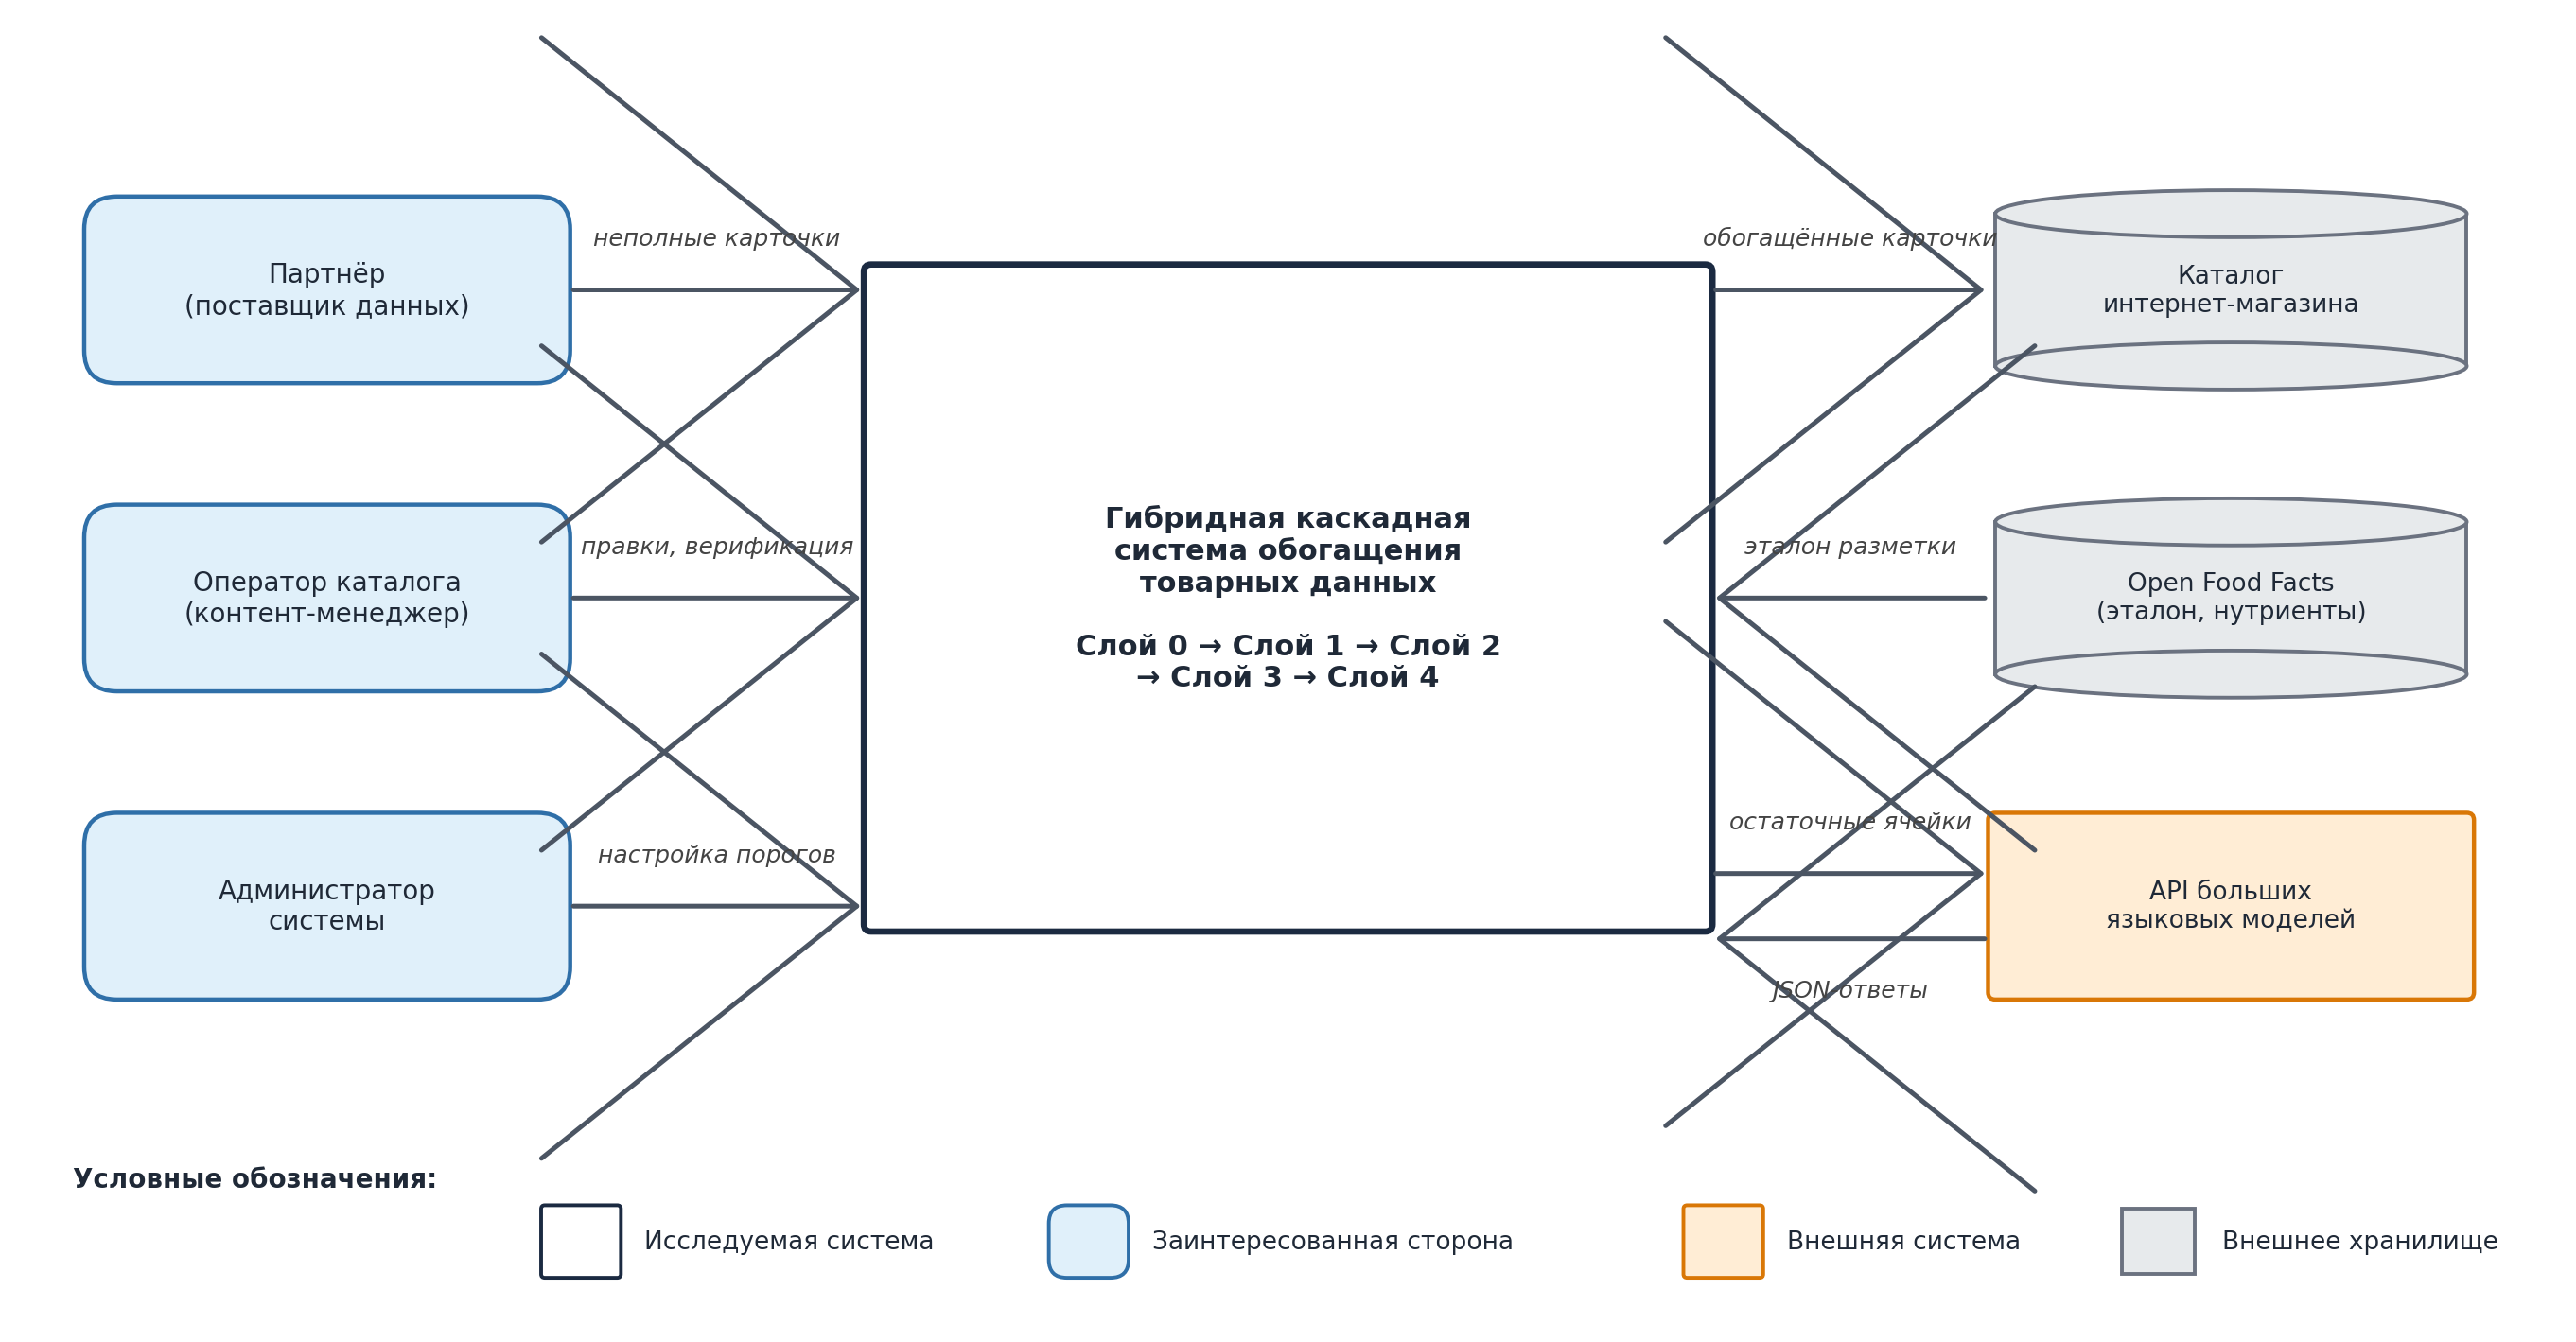
\includegraphics[height=5.7cm]{gost_architecture.png}

\vspace{0.3em}
\fontsize{10pt}{12pt}\selectfont
Контекстная диаграмма: \textbf{система обогащения} между заинтересованными
сторонами (партнёр / оператор / администратор) и внешними системами
(каталог, OFF-эталон, API больших языковых моделей).
\end{frame}

% --- Slide: Архитектура каскадного решения -------------------------------
\begin{frame}{Функциональная модель системы}
\centering

\includegraphics[width=0.93\linewidth]{fig_2_1_functional_model.png}

\vspace{0.2em}
\fontsize{9pt}{11pt}\selectfont
\textbf{Шлюз API (Go)} $\to$ \textbf{ML-сервис (FastAPI)} с каскадом из 5 слоёв.
Каждый слой возвращает $(\hat y, c, \ell)$ или отказ; эскалация — только при низкой уверенности.
\end{frame}

% ===========================================================================
\section{Алгоритмы}
% ===========================================================================

% --- Slide: Ключевые алгоритмы каскада -----------------------------------
\begin{frame}{Ключевые алгоритмы каскада}
\centering
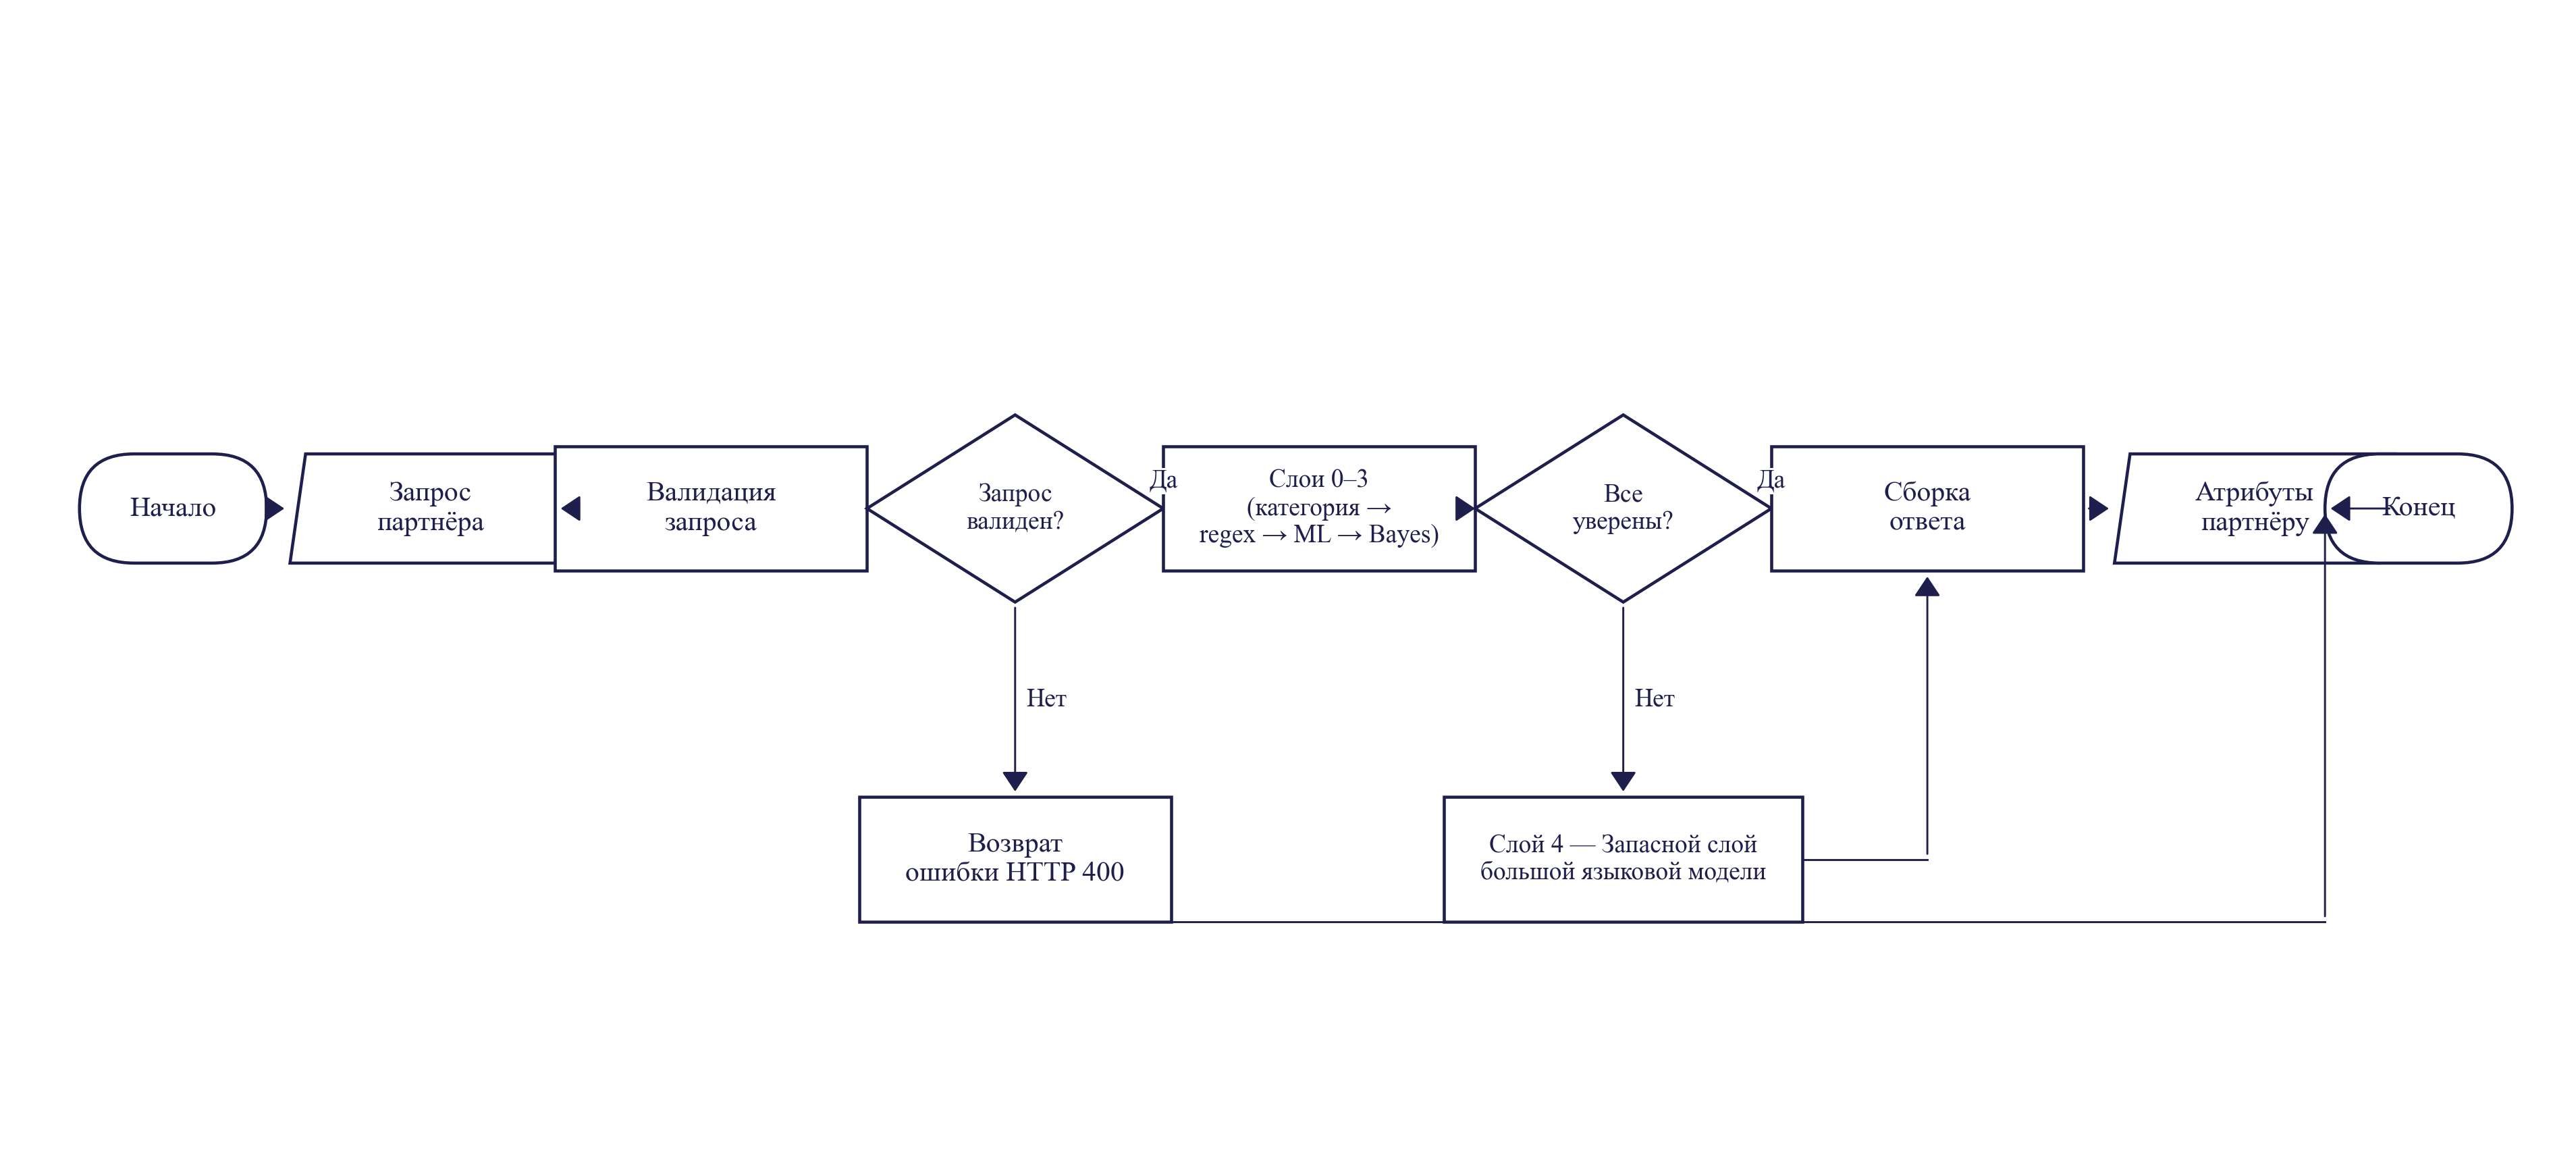
\includegraphics[width=0.94\linewidth]{fig_3_1_algorithm_flowchart_landscape.png}

\vspace{0.3em}
\fontsize{9.5pt}{11.5pt}\selectfont
\textbf{Решение слоя:} $\hat y$, если $p_{\max}(x) \ge \theta_{c,a}$ (поатрибутный порог,
Platt + isotonic). Иначе — эскалация. \textbf{LLM} вызывается на 7{,}1\,\% ячеек.
\end{frame}

% ===========================================================================
\section{Данные и методология}
% ===========================================================================

% --- Slide: Данные и протокол оценки -------------------------------------
\begin{frame}{Данные и протокол оценки}
\begin{columns}[T]
\column{0.55\textwidth}
\fontsize{11pt}{13pt}\selectfont
\textbf{Источник:} Open Food Facts, 4{,}5\,млн SKU
($\sim$40\,\% FR\,/\,10\,\% EN\,/\,7\,\% DE).

\vspace{0.5em}
\textbf{3 категории:} паста (8 атр.), шоколад (7), сыры (7) —
\textbf{22 пары} «категория-атрибут».

\vspace{0.5em}
\textbf{Эталон:} два уровня — основной ($n = 3257$, majority vote 3 LLM)
и HUMAN gold ($n = 615$, консервативная граница).

\vspace{0.5em}
\textbf{Протокол:} проверка на непересекающихся брендах. Pre-registration H1 (router):
\texttt{cd9ac7a} (2026-05-13).

\column{0.42\textwidth}
\centering
\fontsize{8pt}{9pt}\selectfont
\setlength{\tabcolsep}{3pt}
\begin{tabular}{lr}
\toprule
\textbf{Категория} & \textbf{Атрибутов} \\
\midrule
Pasta            & 8 \\
Chocolate        & 7 \\
Cheeses          & 7 \\
\midrule
\textit{Расширения:} & \\
Beverages        & 8 \\
Cereals          & 8 \\
Cosmetics        & 6 \\
\midrule
\textit{Cold-start:} & \\
Electronics      & 8 \\
\bottomrule
\end{tabular}
\end{columns}
\end{frame}

% ===========================================================================
\section{Результаты}
% ===========================================================================

% --- Slide: Главный результат --------------------------------------------
\begin{frame}{Главный результат: точность и стоимость}
\centering
\fontsize{10pt}{12pt}\selectfont
\setlength{\tabcolsep}{8pt}
\renewcommand{\arraystretch}{1.15}
\begin{tabular}{lcc}
\toprule
\textbf{Метрика} & \textbf{Значение} & \textbf{$n$} \\
\midrule
\rowcolor{green!10}
\textbf{Cascade-only micro-accuracy} & \textbf{94{,}8\,\%} & 3257 \\
\rowcolor{green!10}
\textbf{Cascade-only macro-F1} & \textbf{0{,}899} & 3257 \\
Router accuracy (per product code) & 95{,}4\,\% & 570 \\
E2E coverage & 96{,}0\,\% & 3257 \\
\rowcolor{green!10}
\textbf{E2E (None=wrong) — production-realistic} & \textbf{91{,}1\,\%} & 3257 \\
\midrule
HUMAN gold (консервативная граница) — E2E & 87{,}5\,\% & 615 \\
\bottomrule
\end{tabular}

\vspace{0.5em}
\fontsize{9.5pt}{11.5pt}\selectfont
Проверка на непересекающихся брендах.\quad
\textbf{Доля LLM: 7{,}1\,\%} ячеек $\Rightarrow$ сокращение стоимости \pos{$\div$14} vs all-LLM baseline.
\end{frame}

% --- Slide: За счёт чего ---------------------------------------------------
\begin{frame}{За счёт чего: вклад слоёв по 22 атрибутам}
\centering
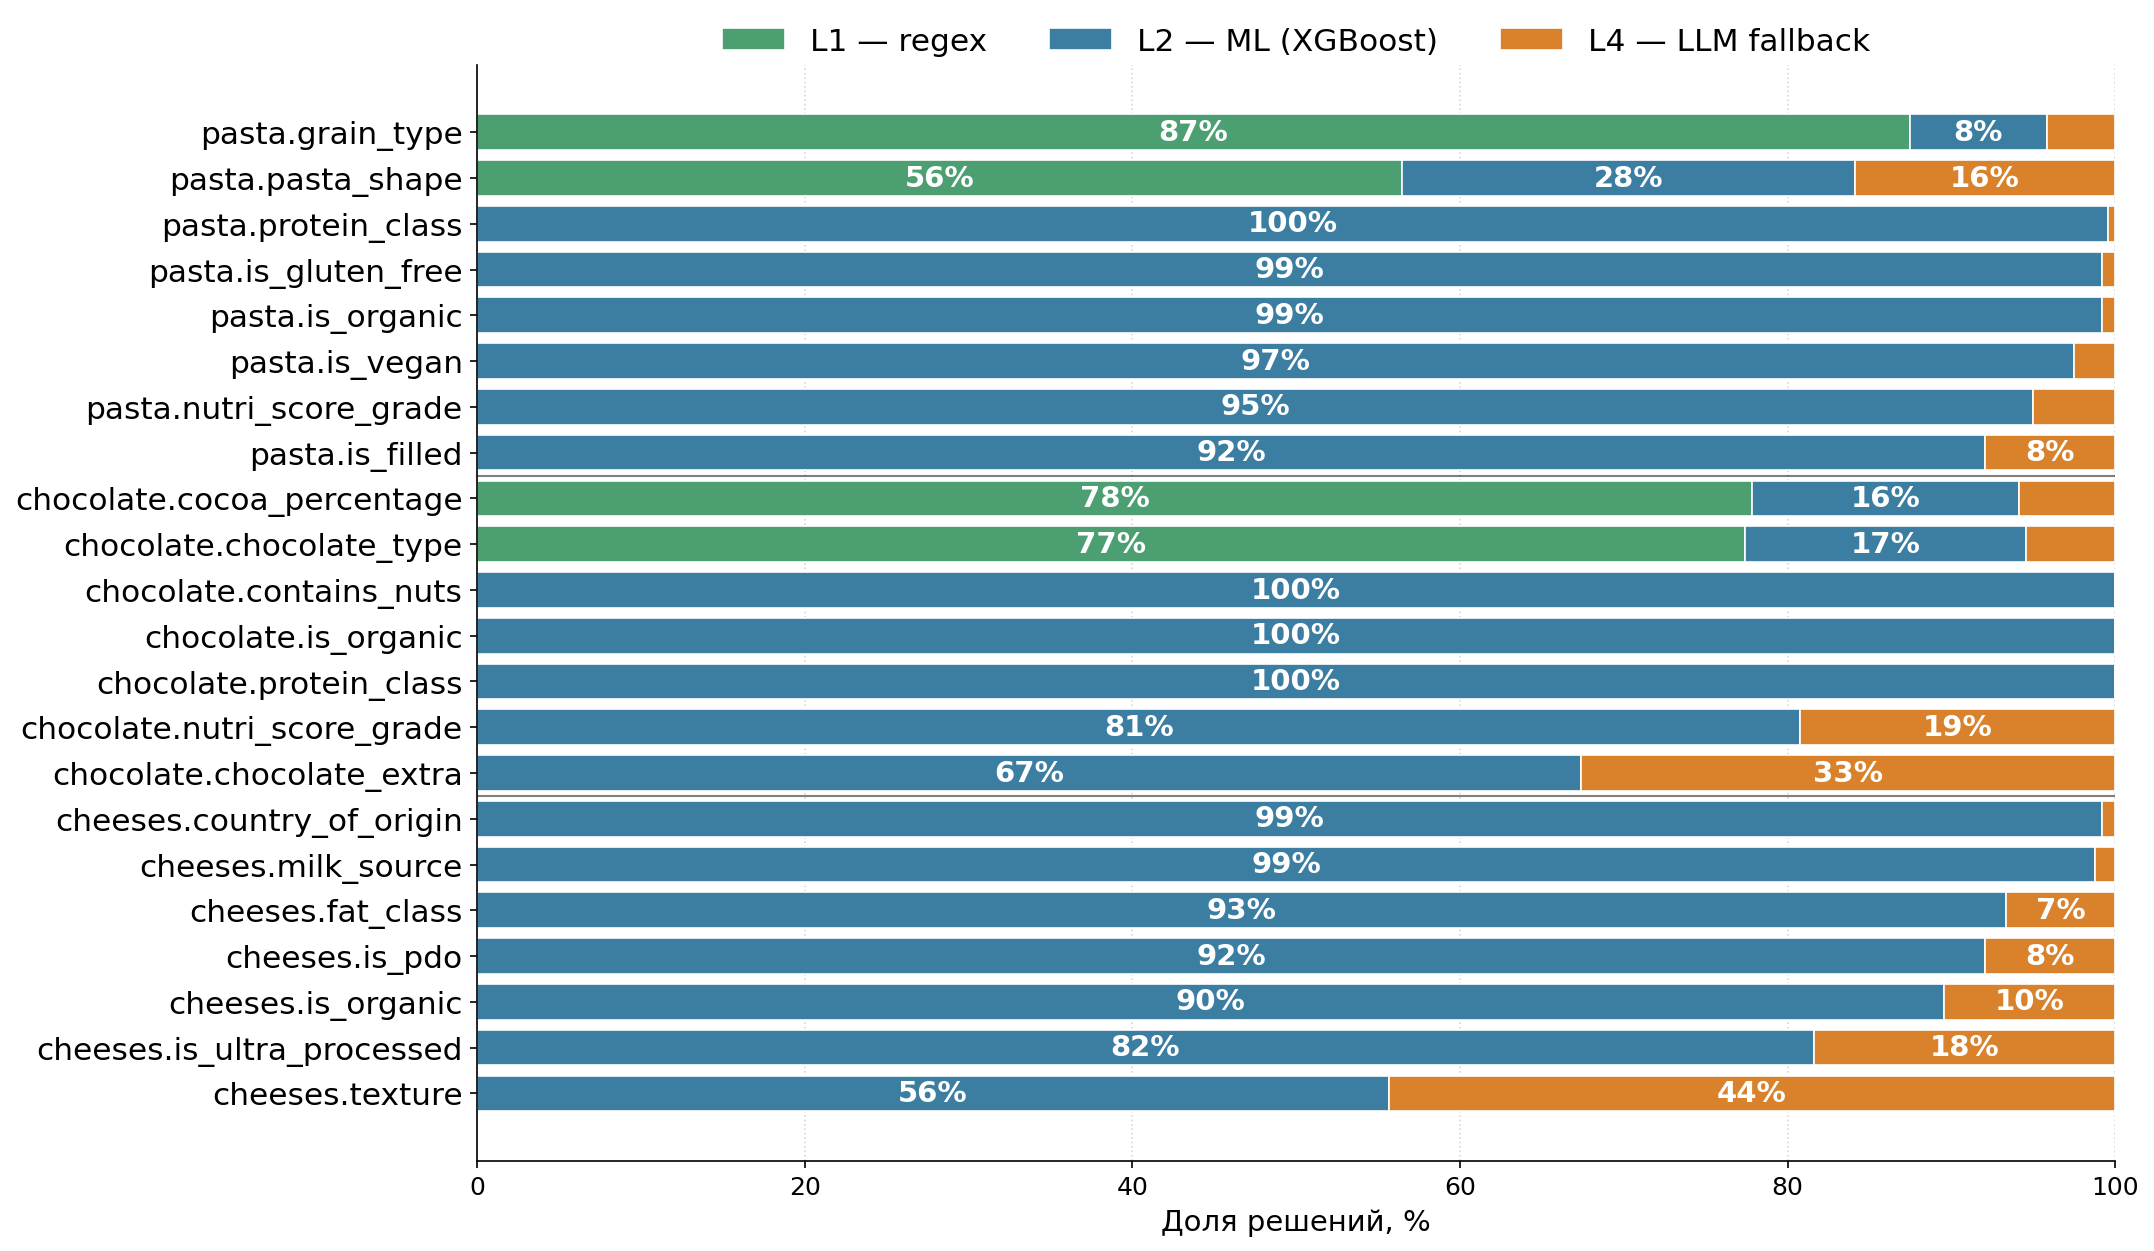
\includegraphics[width=0.95\linewidth]{layer_per_attribute.png}
\end{frame}

% --- Slide: Результаты разработки ПО -------------------------------------
\begin{frame}{Результаты разработки программного средства}
\fontsize{11pt}{14pt}\selectfont
\begin{enumerate}
    \setlength{\itemsep}{0.4em}
    \item \textbf{Соответствие требованиям.}
          Все 6 ФР, 4 НФР, 3 А реализованы; \textbf{4/4 показателя качества}
          достигли целевых.
    \item \textbf{Объём.} $\sim$15\,тыс. строк Python; 35+ модулей; 7 категориальных схем; 22 пары.
    \item \textbf{Демо.} \texttt{docker-compose}: React + Go + FastAPI;
          5 REST-эндпоинтов; $\sim$200\,мс на запрос.
    \item \textbf{Воспроизводимость.} $\sim$70 тестов; ноутбук как исполняемый §3.3;
          \texttt{reproduce.sh} восстанавливает headline-цифры.
\end{enumerate}
\end{frame}

% ===========================================================================
\section{Значимость}
% ===========================================================================

% --- Slide: Научная и практическая значимость ----------------------------
\begin{frame}{Научная и практическая значимость}
\fontsize{10.5pt}{13pt}\selectfont
\textbf{Научная значимость.}
\begin{itemize}
    \setlength{\itemsep}{0.15em}
    \item Методика гибридного каскада с \textbf{поатрибутной калиброванной уверенностью}
          и \textbf{pre-registered} протоколом оценки.
    \item Cascade-only \pos{94{,}8\,\%}\,/\,\pos{0{,}899} macro-F1, E2E \pos{91{,}1\,\%}
          при \pos{$\div$14} стоимости vs all-LLM.
    \item Pre-registered \textbf{отказ} от гипотезы об обучаемом router'е.
    \item Воспроизведено на cold-start (\texttt{electronics}).
\end{itemize}

\vspace{0.5em}
\textbf{Практическая значимость.}
\begin{itemize}
    \setlength{\itemsep}{0.15em}
    \item Работающее ПО в \texttt{docker-compose} рядом с PIM.
    \item Кратное сокращение стоимости и ручной нагрузки.
    \item Локальное развёртывание — независимость от внешних API.
\end{itemize}
\end{frame}

% --- Slide: Достоверность и обоснованность -------------------------------
\begin{frame}{Достоверность и обоснованность результатов}
\fontsize{10.5pt}{13pt}\selectfont
\textbf{Достоверность:}
\begin{itemize}
    \setlength{\itemsep}{0.1em}
    \item проверка на непересекающихся брендах: основная $n{=}3257$ + HUMAN gold $n{=}615$ (две границы);
    \item \textbf{pre-registration} протокола H1 (router) в git \texttt{cd9ac7a} до создания артефакта;
    \item Wilson 95\,\% CI на всех headline-числах;
    \item McNemar + поправка Бонферрони ($\alpha/3$);
    \item воспроизведение через \texttt{reproduce.sh}.
\end{itemize}

\vspace{0.4em}
\textbf{Обоснованность.} Признанные методы:
sentence-transformers, XGBoost, байесовские сети, калибровка Platt + isotonic;
сравнение с TXtract, MAVE, OpenTag, FrugalGPT, AutoMix.

\vspace{0.4em}
\textbf{Реализация.} \texttt{docker-compose} stack с REST API и Web-UI;
код и \texttt{reproduce.sh} опубликованы в репозитории.
\end{frame}

% ===========================================================================
\section{Применение}
% ===========================================================================

% --- Slide: Демонстрационный комплекс ------------------------------------
\begin{frame}{Демонстрационный комплекс — экранные формы}
\centering
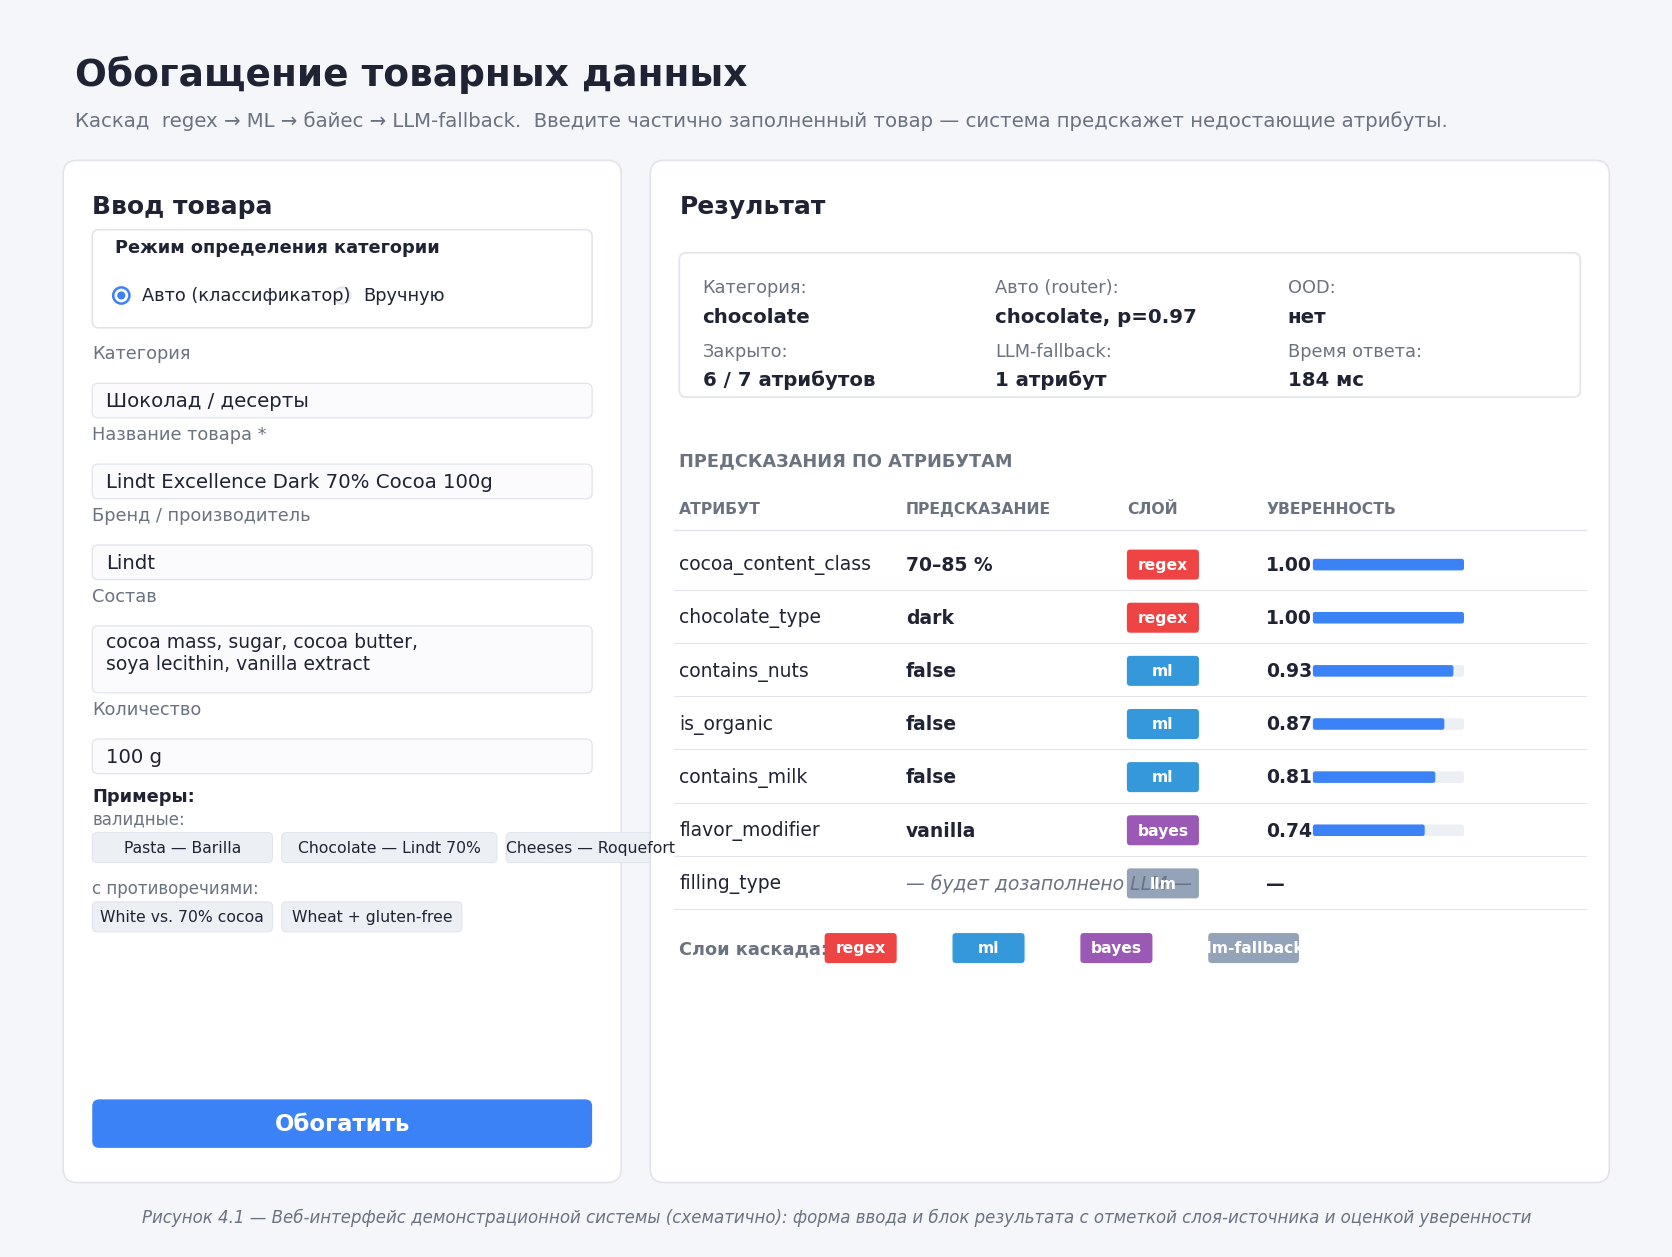
\includegraphics[height=5.5cm]{fig_4_1_demo_ui.png}

\vspace{0.3em}
\fontsize{9pt}{11pt}\selectfont
% TODO (pre-bake): заменить на реальные скриншоты pasta / chocolate / cheeses
% из работающего ml_service. См. spec §7.3.
Стек \textbf{frontend} (React) ↔ \textbf{gateway} (Go) ↔
\textbf{ml\_service} (FastAPI). Для каждой ячейки — значение,
слой-источник и калиброванная уверенность; время ответа $\sim 200$\,мс.
\end{frame}

% --- Slide: Рекомендации -------------------------------------------------
\begin{frame}{Рекомендации по внедрению, эксплуатации и развитию}
\fontsize{10pt}{12.5pt}\selectfont
\begin{columns}[T]
\column{0.32\textwidth}
\textbf{Внедрение}
\begin{itemize}
    \setlength{\itemsep}{0.2em}
    \item \texttt{docker-compose up} рядом с PIM.
    \item Стартовый silver-эталон из истории каталога.
    \item Per-attribute пороги через JSON-конфиги.
    \item LLM: внешний API или локальный Ollama.
\end{itemize}

\column{0.32\textwidth}
\textbf{Эксплуатация}
\begin{itemize}
    \setlength{\itemsep}{0.2em}
    \item Мониторинг доли LLM ($\le 10\,\%$).
    \item Точность на сэмпле $n \ge 200$ еженедельно.
    \item Аудит при росте Bayes-флагов $> 5\,\%$.
    \item Верификация только флагированных ячеек.
\end{itemize}

\column{0.32\textwidth}
\textbf{Развитие}
\begin{itemize}
    \setlength{\itemsep}{0.2em}
    \item Cold-start на новые категории.
    \item Расширение схем атрибутов.
    \item Апгрейд backbone-эмбеддинга.
    \item Подключение более дешёвых LLM.
\end{itemize}
\end{columns}
\end{frame}

% --- Slide: Оперативный эффект -------------------------------------------
\begin{frame}{Оперативный эффект от внедрения}
\fontsize{10pt}{12pt}\selectfont
\vspace{0.5em}
\begin{columns}[c]
\column{0.245\textwidth}\centering
{\fontsize{28pt}{28pt}\selectfont\bfseries\color{posgreen}94{,}8\,\%}\\[0.5em]
\fontsize{9pt}{11pt}\selectfont
cascade-only acc\\(consensus, $n{=}3257$)

\column{0.245\textwidth}\centering
{\fontsize{28pt}{28pt}\selectfont\bfseries\color{posgreen}91{,}1\,\%}\\[0.5em]
\fontsize{9pt}{11pt}\selectfont
E2E production-\\realistic accuracy

\column{0.245\textwidth}\centering
{\fontsize{28pt}{28pt}\selectfont\bfseries\color{posgreen}7{,}1\,\%}\\[0.5em]
\fontsize{9pt}{11pt}\selectfont
доля ячеек,\\эскалированных на LLM

\column{0.245\textwidth}\centering
{\fontsize{28pt}{28pt}\selectfont\bfseries\color{posgreen}$\div$14}\\[0.5em]
\fontsize{9pt}{11pt}\selectfont
сокращение стоимости\\vs all-LLM baseline
\end{columns}

\vspace{1.4em}
\centering
\fontsize{10pt}{12pt}\selectfont\itshape\color{black!65}
$\Rightarrow$ кратное сокращение ручной нагрузки и стоимости обогащения\\
при сохранении локального развёртывания.
\end{frame}

% ===========================================================================
\section{Заключение}
% ===========================================================================

% --- Slide: Заключение (таблица задача → результат) ----------------------
\begin{frame}{Заключение: задачи и полученные результаты}
\centering
\fontsize{9pt}{11pt}\selectfont
\setlength{\tabcolsep}{6pt}
\renewcommand{\arraystretch}{1.2}
\begin{tabular}{p{0.30\linewidth}p{0.66\linewidth}}
\toprule
\textbf{Задача} & \textbf{Результат} \\
\midrule
1. Анализ подходов          & Пробел: hybrid + per-attr + pre-registered eval. \\
2. Требования и качество    & 6 ФР, 4 НФР, 3 А; критерий $Q$ — все цели достигнуты. \\
3. Каскад и маршрутизация   & 4 слоя, 22 пары $\times$ 3 категории, калиброванные пороги. \\
4. Реализация               & \texttt{docker-compose} + REST + Web-UI; $\sim$15\,тыс. строк Python. \\
5. Pre-registered оценка    & $n{=}3257$: cascade \pos{94{,}8\,\%}\,/\,\pos{0{,}899} mF1, E2E \pos{91{,}1\,\%}, \pos{$\div$14} cost; H1 отвергнута. \\
6. Рекомендации             & Внедрение / эксплуатация / развитие; cold-start. \\
\bottomrule
\end{tabular}

\vspace{0.6em}
\fontsize{10.5pt}{13pt}\selectfont
\textbf{Итог:} cascade-only \textbf{94{,}8\,\%} / 0{,}899 macro-F1, E2E \textbf{91{,}1\,\%}
при \pos{$\div$14} стоимости vs all-LLM.
\end{frame}

% --- Slide: Спасибо ------------------------------------------------------
\begin{frame}{Спасибо за внимание}
\begin{columns}[c]
\column{0.55\textwidth}
\fontsize{11pt}{13pt}\selectfont
Исходный код, ноутбук §3.3 в исполняемом виде, демонстрационный
комплекс и текст работы доступны в репозитории проекта.

\vspace{1em}
\large Вопросы?

\column{0.42\textwidth}
\centering

\includegraphics[height=4.5cm]{qr-git.pdf}\\
\fontsize{8pt}{10pt}\selectfont
\texttt{github.com/Qworl/diploma}
\end{columns}
\end{frame}

% ===========================================================================
\appendix
\backupbegin
% ===========================================================================

% --- B1 ------------------------------------------------------------------
\begin{frame}{B1. Отрицательный результат: обучаемый router}
\begin{columns}[T]
\column{0.5\textwidth}
\fontsize{9pt}{11pt}\selectfont
\textbf{Гипотеза H1:} обучаемый стоимостно-чувствительный маршрутизатор
превосходит статическое правило хотя бы на одном из трёх бюджетов LLM
(25\,\% / 40\,\% / 50\,\%).

\vspace{0.3em}
\textbf{Pre-registration:} git \texttt{cd9ac7a}, 2026-05-13 02:11
(за 1\,ч\,11\,мин до создания артефакта).

\vspace{0.3em}
\textbf{Поправка Бонферрони:} $\alpha/3 \approx 0{,}0167$.

\textbf{MDE на $n=1539$:} $\approx 4{,}4$\,пп (парный McNemar).

\textbf{Результат:} $p > 0{,}3$ во всех трёх бюджетах.

\column{0.48\textwidth}
\centering
\fontsize{8pt}{9pt}\selectfont Pareto: router vs static\\
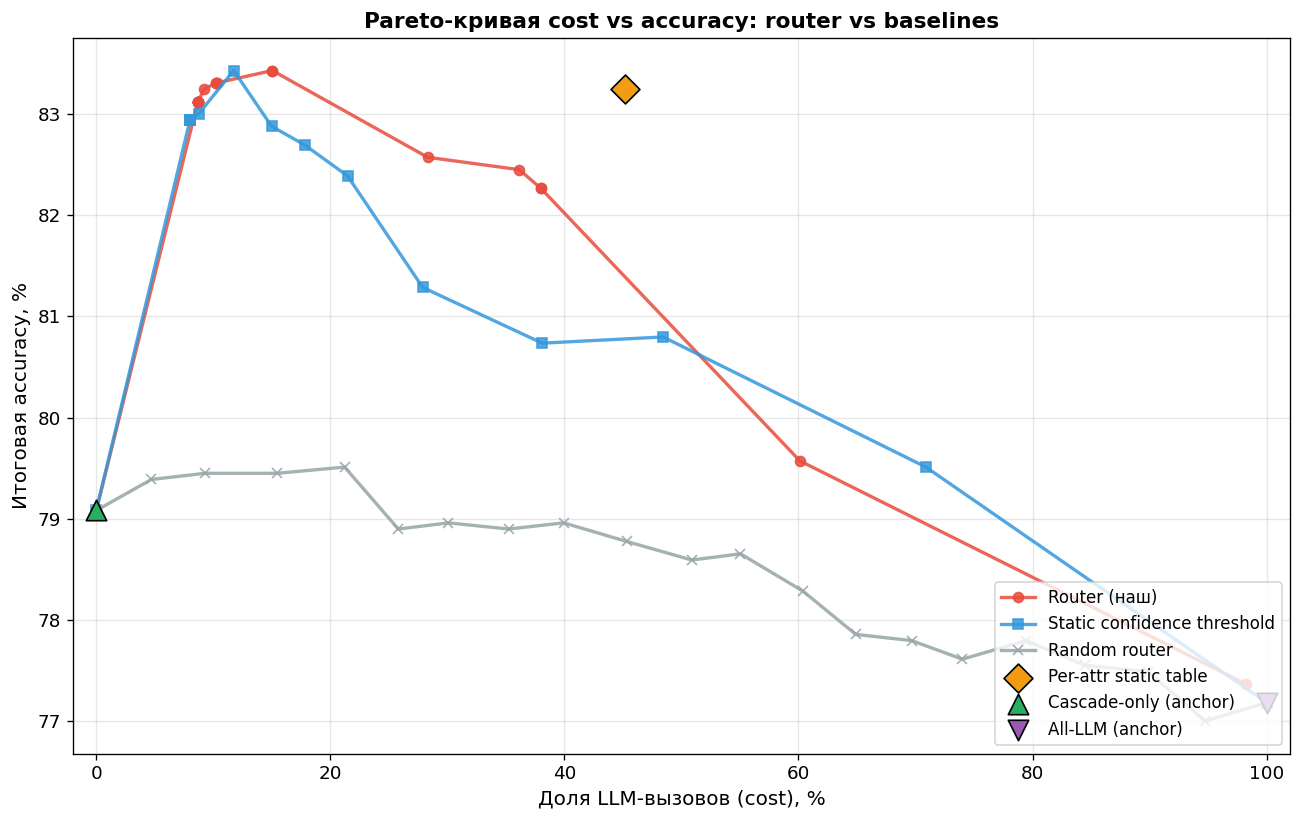
\includegraphics[width=\linewidth]{router_pareto_curve.png}
\end{columns}
\end{frame}

% --- B2 ------------------------------------------------------------------
\begin{frame}{B2. Селективное поведение Bayes-валидатора}
\begin{columns}[T]
\column{0.55\textwidth}
\fontsize{9pt}{11pt}\selectfont
Bayes-валидатор активен \textbf{селективно} — флаг ставится только при
$q_{c,a}$-калибровке плотностей, выбран per-attr пороги
(см. \texttt{*\_validation\_thresholds.json}).

\vspace{0.3em}
\textbf{Hybrid CPD-fit:} структура DAG — Hill Climb + BIC на silver
(15K с непересекающимися брендами vs test); CPD — на
\texttt{CONCAT(silver, gold-train × 10)} с BDeu prior.

\vspace{0.3em}
\textbf{Production:} 10 useful Bayes-пар, селективное флагирование на
\textit{chocolate/contains\_nuts}, \textit{cheeses/is\_ultra\_processed} и др.

\column{0.42\textwidth}
\centering
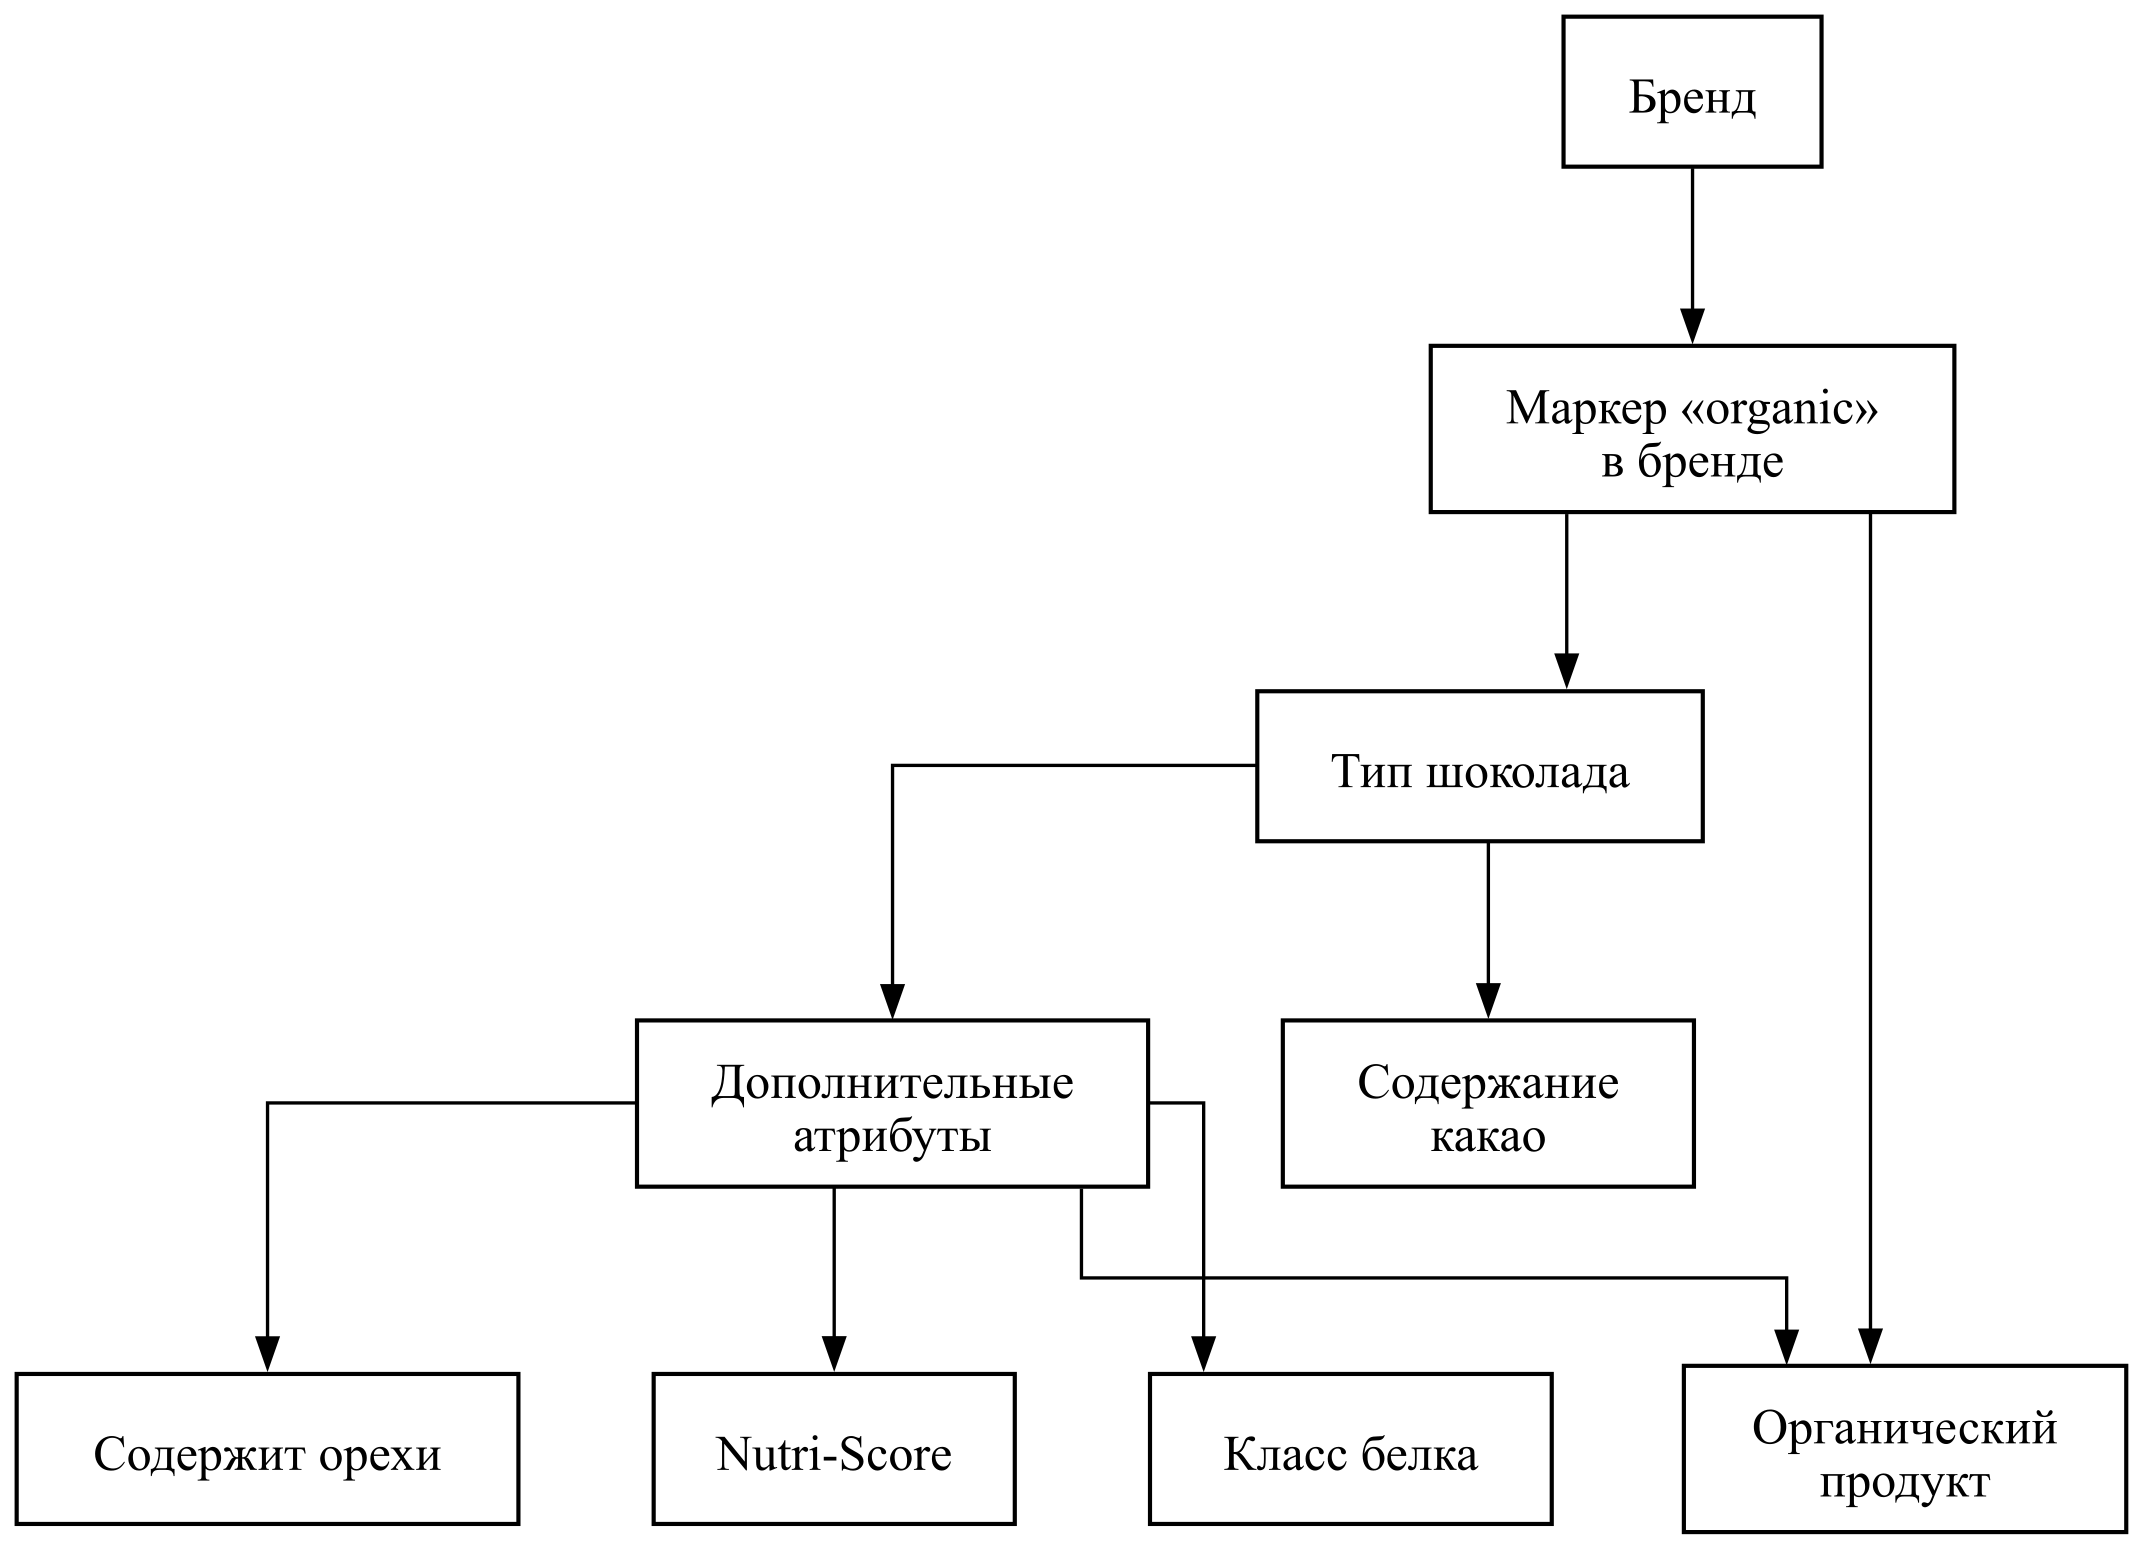
\includegraphics[height=5.5cm]{fig_3_5_bayes_dag.png}
\end{columns}
\end{frame}

% --- B3 ------------------------------------------------------------------
\begin{frame}{B3. Silver vs Gold standard}
\fontsize{10pt}{12pt}\selectfont
\textbf{Silver standard} (consensus тегов OFF + 3 LLM + слепая Opus-разметка)
служит \textbf{обучающим} сигналом. Gold-эталон (\texttt{consensus\_gold\_v2\_expanded.parquet})
получен по аудит-циклу для холдаута.

\vspace{0.3em}
\textbf{Цикл «аудит — правки экстрактора — переобучение — измерение»} воспроизведён
3 из 3 категорий с приростом \pos{+18{,}2}, \pos{+16{,}3}, \pos{+14{,}4}\,пп.

\vspace{0.3em}
\textbf{Калибровка уверенности} — комбинация Platt + isotonic
per (категория, атрибут); ECE измеряется на отдельной выборке,
артефакты сохраняются в \texttt{*\_calibration.json}.
\end{frame}

% --- B4 ------------------------------------------------------------------
\begin{frame}{B4. Утечки и борьба с ними}
\fontsize{10pt}{12pt}\selectfont
\textbf{Запрет утечки \texttt{categories\_tags} в эмбеддинги.}

Эмбеддинги Слоя~2 строятся \textbf{только} из partner-available полей:
\texttt{product\_name + brands + ingredients\_text + quantity}.
\texttt{categories\_tags} — это \textit{выход} обогащения, не вход;
использование как фичи привело бы к target leakage.

\vspace{0.3em}
\textbf{Brand-disjoint split (60/20/20).} Бренды в train/val/test
\textbf{не пересекаются} — гарантия обобщения на новых брендах.

\vspace{0.3em}
\textbf{k-NN ablation (§3.3.7.3):} точность \textbf{не падает} на удалённых от обучающей
выборки товарах — монотонный рост от Q1 (82{,}7\,\%) до Q4 (91{,}6\,\%).
\end{frame}

% --- B5 ------------------------------------------------------------------
\begin{frame}{B5. Мультиязычность}
\fontsize{10pt}{12pt}\selectfont
\textbf{Языковой состав OFF:} $\approx$40\,\% FR, 10\,\% EN, 7\,\% DE, остальное — прочие.

\vspace{0.3em}
\textbf{Эмбеддинг:} \texttt{paraphrase-multilingual-MiniLM-L12-v2}
(50+ языков, общее семантическое пространство).

\vspace{0.3em}
\textbf{Поатрибутно-поязыковой срез} (\texttt{per\_language\_eval.parquet},
132 записи на $n{=}3257$ ячейках): взвешенная точность стабильна по основным языкам.

\vspace{0.3em}
\textbf{Под балансировку каскад не оптимизировался} — это естественный
выигрыш многоязычного backbone'а.
\end{frame}

% --- B6 ------------------------------------------------------------------
\begin{frame}{B6. LLM-cost на 1M~SKU}
\fontsize{10pt}{12pt}\selectfont
\textbf{Каскад делегирует LLM лишь $7{,}1$\,\% ячеек} ($n=3506$) —
прямая прокси к стоимости. Cost reduction \textbf{92{,}9\,\% ($\div$14)}
относительно «прямой LLM на всё».

\vspace{0.3em}
\textbf{Распределение по слоям:}
\fontsize{9pt}{11pt}\selectfont
L1 (regex high-precision) — 18{,}4\,\%, L2 (ML) — \textbf{73{,}8\,\%},
L3 (regex low-precision) — 0{,}7\,\%, L4 (LLM) — 7{,}1\,\%.

\vspace{0.3em}
\fontsize{10pt}{12pt}\selectfont
\textbf{Проекция на 1M SKU × 22 атрибута} ($\sim 2{,}2\cdot 10^7$ ячеек):
\begin{itemize}
    \fontsize{9pt}{11pt}\selectfont
    \setlength{\itemsep}{0.15em}
    \item Прямой LLM — оплачены все $\sim 2{,}2\cdot 10^7$ вызовов.
    \item Каскад — оплачены лишь $\sim 1{,}6\cdot 10^6$ вызовов ($7{,}1\,\%$).
\end{itemize}

\vspace{0.2em}
\textbf{Топ-3 LLM-затратных атрибутов:}
pasta.grain\_type (32{,}9\,\%), pasta.pasta\_shape (22{,}8\,\%), cheeses.is\_pdo (13{,}6\,\%).
\end{frame}

% --- B7 ------------------------------------------------------------------
\begin{frame}{B7. Cold-start: electronics (§5 ноутбука)}
\begin{columns}[T]
\column{0.55\textwidth}
\fontsize{9pt}{11pt}\selectfont
Демонстрация переноса методологии на \textbf{новую категорию без regex-правил}.

\vspace{0.3em}
\textbf{Электроника (8 атрибутов):}
смартфоны — RAM, storage, screen size, has 5G, …

\vspace{0.3em}
\textbf{Transfer:} только Слой~2 (ML+эмбеддинги) и Слой~4 (LLM);
Слой~1 пропускается; Слой~3 — по обучающим парам.

\vspace{0.3em}
\textbf{Результат:} cold-start работает на small-shot, обоснованность
расширения каскада за пределы food-доменов.

\column{0.42\textwidth}
\centering
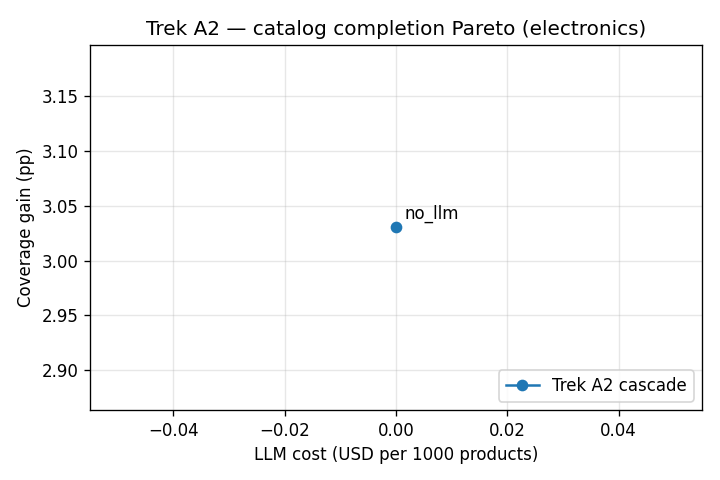
\includegraphics[width=\linewidth]{trek_a2_pareto_electronics.png}
\end{columns}
\end{frame}

\backupend

\end{document}
